\documentclass[a4paper, 12pt]{article}%тип документа

%отступы
\usepackage[left=2cm,right=2cm,top=2cm,bottom=3cm,bindingoffset=0cm]{geometry}

%Русский язык
\usepackage[T2A]{fontenc} %кодировка
\usepackage[utf8]{inputenc} %кодировка исходного кода
\usepackage[english,russian]{babel} %локализация и переносы

%Вставка картинок
\usepackage{graphicx}
\graphicspath{{pictures/}}
\DeclareGraphicsExtensions{.pdf,.png,.jpg}

%Графики
\usepackage{pgfplots}
\pgfplotsset{compat=1.9}

%Математика
\usepackage{amsmath, amsfonts, amssymb, amsthm, mathtools}

%Римские цифры
\newcommand{\RomanNumeralCaps}[1]{\uppercase\expandafter{\romannumeral#1}}

%Таблицы
\usepackage{longtable}

\begin{document}
	\begin{titlepage}
		\begin{center}
			\textsc{Федеральное государственное автономное образовательное учреждение высшего образования«Московский физико-технический институт (национальный исследовательский университет)»\\[5mm]
			}
			
			\vfill
			
			\textbf{Отчет по лабораторной работе 1.2.1\\[3mm]
				Определение скорости полета пули при помощи баллистического маятника.
				\\[50mm]
			}
		\end{center}
		
		\hfill
		\begin{minipage}{.5\textwidth}
			Выполнил студент:\\[2mm] 
			Сериков Василий Романович\\[2mm] 
			группа: Б03-102\\[5mm]
			
		\end{minipage}
		\vfill
		\begin{center}
			Москва, 2021 г.
		\end{center}
	\end{titlepage}
	
	\newpage
	\textbf{Цель работы:} Определить скорость полета пули, применяя законы сохранения и используя баллистические маятники.\\
	\textbf{В работе используется:} Духовое ружье на штативе, осветитель, оптическая система для измерения отклонений маятника, измерительная линейка, пули и весы для их взвешивания, баллистические маятники. \\
	\textbf{Теория:} Баллистическим называется маятник, колебания которого вызываются кратковременным начальным импульсом. Необходимо позаботиться, чтобы после удара пули колебания маятника происходили в одной плоскости и отсутствовали поперечные движения.
	\RomanNumeralCaps{1} метод определения скорости пули - это метод с помощью баллистического маятника, совершающего поступательное движение (рис.1). Маятник состоит из цилиндра, подвешенного на 4 нитях одинаковой длины. Расчет скорости пули выполняется по следующей формуле: $$ u=\frac{M}{m} \sqrt{\frac{g}{L}} \Delta x $$ \\
		\begin{figure}[h]
		\center{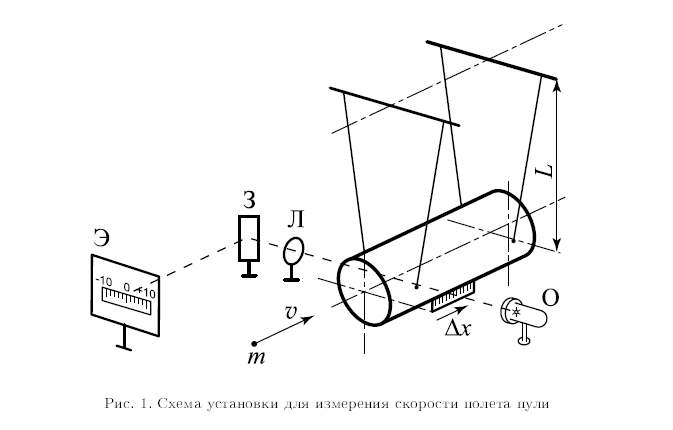
\includegraphics [scale=0.9]{Снимок экрана (433).png}}
	\end{figure}\\
	\RomanNumeralCaps{2} метод измерения скорости пули - это с помощью баллистического маятника, совершающего крутильные колебания (рис.2). Пуля попадает в мишень, которая вместе с грузами и со стержнем составляет крутильный баллистический маятник. Сразу после попадания пули в мишень, система пуля-мишень будет двигаться с угловой скоростью $\Omega$ такой, что
	\begin{equation}
		m v r = I \Omega,
	\end{equation}
	где $I$ -- момент инерции систему пуля-мишень.\\
	Если $k$ -- модуль кручения проволоки, то из закона сохранения энергии следует, что
	\begin{equation}
		k \frac{\varphi^2}{2} = I \frac{\Omega^2}{2},
	\end{equation}
	где $\varphi$ -- амплитуда колебаний маятника после выстрела.
	Из уравнений (4) и (5) можно найти скорость $v$ по амплитуде $\varphi$.
	\begin{equation}
		v = \varphi \frac{\sqrt{kI}}{mr}.
	\end{equation}\\
    где  $\varphi$ = $\frac{x}{2d}$, а d - расстояние от шкалы до оси,  $x$ -- смещение изображения нити осветителя на шкале.\\
    
    Периоды колебаний маятника с грузами и без можно выразить как
    $$T_2 = 2 \pi \sqrt{\frac{I}{k}} \;\;\;\;\;\; T_1= 2 \pi \sqrt{\frac{I - 2MR^2}{k}}$$
    Тогда $\sqrt{kI}$ можно найти как 
    	\begin{equation}
    		\sqrt{kI} = \frac{4 \pi M R^2 T_2}{T_2^2 - T_1^2}
    	\end{equation}
    
    	\begin{figure}[h]
    	\center{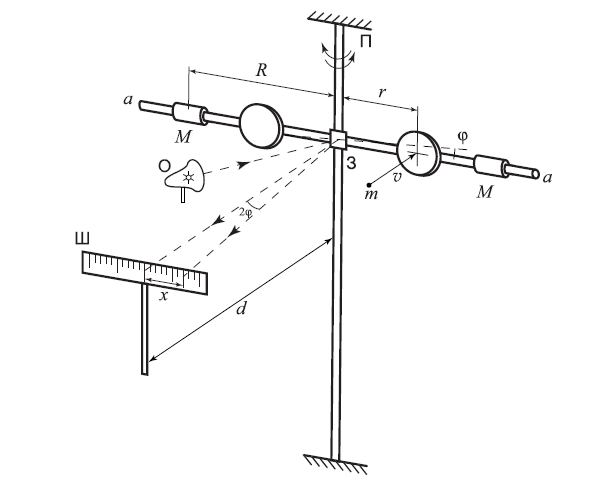
\includegraphics [scale=0.9]{Снимок экрана (435).png}}
    \end{figure}
	\center{\textbf{Рис.2 Схема установки для измерения скорости пули с крутильным баллистическим маятником}}\\
	
	\begin{enumerate}
	\textbf{Ход работы:} \\
	Работа с маятником, совершающим поступательное движение.
	\item Измеряем массы пулек на весах, результаты занесем в таблицу 1. Погрешность измерения массы: $\sigma_m = \pm0,001 \text{ г}$ 
	
		\begin{longtable}{|c|c|c|c|c|c|c|c|c|}
		\hline 
		№ & 1 & 2& 3 & 4 & 5 & 6 & 7 & 8 \\
		\hline
		m, г& 0,512& 0,509& 0,510& 0,516 & 0,502 & 0,514 & 0,504 & 0,515\\
		\hline
		\caption{Массы 8 пулек.}
	\end{longtable}

	\item Измерим расстояние L. L=(220,0$\pm0,1$) см. Масса маятника M=2900 $\pm$5 г
	\item Произведя холостой выстрел, мы убедились, что маятник не реагирует на воздушную струю из ружья.
	\item Мы убедились, что амплитуда при 10 колебаний маятника не уменьшается более, чем в 2 раза.
	\item Произведем 4 выстрела и определим скорость пули в каждом случае по формуле $ u=\frac{M}{m} \sqrt{\frac{g}{L}} \Delta x $ . Полученные данные (x-смещение маятника, u-скорость пули, $\sigma_u$-погрешность измерения скорости) занесем в таблицу 2. \\
	 $\sigma_u = \sqrt{(\frac{\partial f}{\partial M}\sigma_M)^2 + (\frac{\partial f}{\partial m}\sigma_m)^2 + (\frac{\partial f}{\partial L}\sigma_L)^2+(\frac{\partial f}{\partial x}\sigma_x)^2 }$ \\
	  $\sigma_x$  = $\pm$0,5 мм
	 
	 	\begin{longtable}{|c|c|c|c|c|}
	 	\hline 
	 	№ & 1 & 2 & 3 & 4 \\
	 	\hline
	 	x, мм &13,5 &13,2 &13,2  &13,4 \\
	 	\hline
	 	u, м/с &161 & 158 & 158 & 158\\
	 	\hline 
	 	$\sigma_u$, м/с &5 &5 &5 &5 \\
	 	\hline 
	 	\caption{Значения x, u, $\sigma_u$ для 4 пулек. }
	 \end{longtable}
 
 
	\item Посчитаем среднее значение скорости. Таким образом: $\overline{u}$ = 159 $\pm 5$ м/с
\end{enumerate}
	

		\textbf{Работа с крутильным баллистическим маятником.}
		\begin{enumerate}
			
		\item Измерим значения r, R, d. r =(23,0 $\pm 0,1$) см, R =(33,5 $\pm 0,1$) см, d=(45,0 $\pm 0,1$) см. Значения массы пулек указаны в таблице 1. Масса груза M = 714,1 г.
		\item Измерим время 10 колебаний маятника с грузами и без них, и определим периоды $T_1$ и $T_2$. Полученные данные занесем в таблицу 3.
		\begin{longtable}{|c|c|c|c|}
			\hline 
			$T_1$ & $T_2$  & $\sigma_{T_1}$ & $\sigma_{T_2}$ \\
			\hline
			17,99 c&13,77 c& 0,03 c & 0,03 c\\
			\hline
			\caption{Значения $T_1$, $T_2$, $\sigma_{T_1}$, $\sigma_{T_2}$   }
		\end{longtable}
		\item Найдем величину $\sqrt{kI}$ по формуле $\sqrt{kI} = \frac{4 \pi M R^2 T_2}{T_2^2 - T_1^2}$ и оценим погрешность по формуле:\\ $\sigma_{\sqrt{kI}}= \sqrt{(\frac{\partial f}{\partial R}\sigma_R)^2 + (\frac{\partial f}{\partial T_1}\sigma_{T_1})^2 + (\frac{\partial f}{\partial T_2}\sigma_{T_2})^2}$. Тогда получим:
		$\sqrt{kI}$ = (0,135 $\pm0,009$)$\frac {\text {кг}\cdot \text{м}^2}{\text{c}}$
		\item Определим скорость четырех пулек при каждом выстреле по формуле $v = \frac{x}{2d}  \frac{\sqrt{kI}}{mr}$. Оценим погрешность по формуле: $\sigma_u = u\sqrt{\left( \dfrac{\sigma_{x}}{x} \right)^2 + \left( \dfrac{\sigma_{d}}{d} \right)^2 + \left( \dfrac{\sigma_{ \sqrt{kI}}}{\sqrt{kI}} \right)^2 + \left( \dfrac{\sigma_{m}}{m} \right)^2+ \left( \dfrac{\sigma_{r}}{r} \right)^2}$. Данные занесем в таблицу 4.
		
		\begin{longtable}{|c|c|c|c|c|}
			\hline 
			№ & 1 & 2 & 3 & 4 \\
			\hline
			x, см &12,5 &12,8 &12,5  &12,4 \\
			\hline
			u, м/с &162 & 162 & 161 & 157\\
			\hline 
			$\sigma_u$, м/с &2 &2 &2 &2 \\
			\hline 
			\caption{Значения x, u, $\sigma_u$ для 4 пулек. }
		\end{longtable}	
	\item  Таким образом среднее значение скорости равно: $\overline{u}$ = 161 $\pm 2$ м/с
	\item \textbf{Вывод:} Применив два способа измерения скорости полета пули, мы получили одинаковые значения скоростей в пределах погрешности.
	
	
	\end{enumerate}
\end{document}